\documentclass{article}

\usepackage{amsmath, amssymb}
\usepackage{multicol}
\usepackage[table]{xcolor}
\usepackage{forest}
\usepackage[a4paper, bindingoffset=0in, left=0.2in, right=0.1in, top=0.1in,
            bottom=0.2in, footskip=0.25in]{geometry}
\usepackage{parskip}
\usepackage{draftwatermark}
\usepackage{enumitem}
\usepackage{multicol}
	
\SetWatermarkColor[gray]{0.95}
\SetWatermarkText{Isaac Boaz}
\SetWatermarkScale{1}

\pagenumbering{gobble}

\begin{document}
\small

\setlist{nosep}
\setlength{\parindent}{0em}
\setlength{\itemindent}{0em}
\setlength{\leftmargini}{0em}

\begin{multicols*}{2}
    \subsection*{General DP Remarks}
    \subsubsection*{Optimal Substructure}
    \begin{itemize}
        \item Create optimal solution to problem using optimal solutions to
              subproblems.
        \item Can't use DP if optimal solution to a problem does not require
              subproblem solutions to be optimal. \\
              \(\rightarrow\) Often happens when subproblems are \emph{not
                  independent} of each other.
    \end{itemize}
    \subsubsection*{Overlapping Subproblems}
    \begin{itemize}
        \item For DP to be useful, recursive algorithm should require us to compute
              optimal solutions to the \emph{same subproblems} over and over again.
        \item In total, there should be a small number of distinct subproblems (i.e.
              polynomial in input size).
    \end{itemize}

    \subsection*{LCS}
    \begin{equation*}
        LCS[i, j] = \begin{cases}
            1 + LCS[i-1, j-1]              & \text{if } x_i = y_i \\
            \max(LCS[i-1, j], LCS[i, j-1]) & \text{otherwise}
        \end{cases}
    \end{equation*}
    \hspace*{-1.5em}
    \begin{tabular}{|c|c|c|c|c|c|c|c|c|c|c|}
        \hline
                                      &                               & j=0                           & j=1                            & j=2
                                      & j=3                           & j=4                           & j=5
                                      & j=6                           & j=7                           & j=8                                                 \\
        \hline
                                      &                               &                               & p                              & r
                                      & i                             & n                             & t
                                      & i                             & n                             & g                                                   \\
        \hline
        i=0                           &                               & 0                             & 0                              & 0
                                      & 0                             & 0                             & 0
                                      & 0                             & 0                             & 0                                                   \\
        \hline
        i=1                           & s                             & 0                             & 0                              & 0
                                      & 0                             & 0                             & 0
                                      & 0                             & 0                             & 0                                                   \\
        \hline
        i=2                           & p                             & 0                             & \cellcolor{red!25} 1$\nwarrow$ & 1$\leftarrow$
                                      & 1$\leftarrow$                 & 1$\leftarrow$                 &
        1$\leftarrow$                 & 1$\leftarrow$                 &
        1$\leftarrow$                 & 1$\leftarrow$                                                                                                       \\
        \hline
        i=3                           & r                             & 0                             & 1$\uparrow$                    & \cellcolor{red!25}
        2$\nwarrow$                   & 2$\leftarrow$                 & 2$\leftarrow$
                                      & 2$\leftarrow$                 & 2$\leftarrow$                 &
        2$\leftarrow$                 & 2$\leftarrow$                                                                                                       \\
        \hline
        i=4                           & i                             & 0                             & 1$\uparrow$                    & 2$\uparrow$
                                      & \cellcolor{red!25}3$\nwarrow$ & 3$\leftarrow$                 &
        3$\leftarrow$                 & 3$\leftarrow$                 &
        3$\leftarrow$                 & 3$\leftarrow$                                                                                                       \\
        \hline
        i=5                           & n                             & 0                             & 1$\uparrow$                    & 2$\uparrow$
                                      & 3$\uparrow$                   & \cellcolor{red!25}4$\nwarrow$ &
        4$\leftarrow$                 & 4$\leftarrow$                 &
        4$\leftarrow$                 & 4$\leftarrow$                                                                                                       \\
        \hline
        i=6                           & g                             & 0                             & 1$\uparrow$                    & 2$\uparrow$
                                      & 3$\uparrow$                   & 4$\uparrow$                   &
        4$\uparrow$                   & 4$\uparrow$                   & 4$\uparrow$
                                      & 5$\nwarrow$                                                                                                         \\
        \hline
        i=7                           & t                             & 0                             & 1$\uparrow$                    & 2$\uparrow$
                                      & 3$\uparrow$                   & 4$\uparrow$                   &
        \cellcolor{red!25}5$\nwarrow$ & 5$\leftarrow$                 &
        5$\leftarrow$                 & 5$\leftarrow$                                                                                                       \\
        \hline
        i=8                           & i                             & 0                             & 1$\uparrow$                    & 2$\uparrow$
                                      & 3$\nwarrow$                   & 4$\uparrow$                   &
        5$\uparrow$                   & \cellcolor{red!25}6$\nwarrow$ &
        6$\leftarrow$                 & 6$\leftarrow$                                                                                                       \\
        \hline
        i=9                           & m                             & 0                             & 1$\uparrow$                    & 2$\uparrow$
                                      & 3$\uparrow$                   & 4$\uparrow$                   &
        5$\uparrow$                   & 6$\uparrow$                   & 6$\uparrow$
                                      & 6$\uparrow$                                                                                                         \\
        \hline
        i=10                          & e                             & 0                             & 1$\uparrow$                    & 2$\uparrow$
                                      & 3$\uparrow$                   & 4$\uparrow$                   &
        5$\uparrow$                   & 6$\uparrow$                   & 6$\uparrow$
                                      & 6$\uparrow$                                                                                                         \\
        \hline
    \end{tabular}

    \subsection*{OBST}
    \begin{equation*}
        e[i, j] = \begin{cases}
            0                                                          & \text{if } i = j - 1 \\
            \min_{i \leq r \leq j} \{e[i, r-1] + e[r+1, j] + w(i, j)\} & \text{if } i \leq j
        \end{cases}
    \end{equation*}
    \begin{equation*}
        root[i, j] = \text{root of subtree with keys } k_i, \ldots, k_j \text{ for } 1 \leq i \leq j \leq n
    \end{equation*}
    \begin{align*}
        w[1, \ldots & , n+1, 0, \ldots, n]  = \text{ sum of probabilities}          \\
                    & w[i, i-1] = 0 \text{ for } 1 \leq i \leq n                    \\
                    & w[i, j] = w[i, j-1] + p_j \text{ for } 1 \leq i \leq j \leq n
    \end{align*}

    Consider 5 keys with search probabilities \(p_1 = 0.25, p_2 = 0.2, p_3 = 0.05,
    p_4 = 0.2, p_5 = 0.3\)

    \hspace*{-1.5em}
    \setlength\tabcolsep{2.5pt}
    % \footnotesize
    \begin{multicols}{2}
        \begin{center}
            \begin{tabular}{c|cccccc}
                w & 0 & 1    & 2    & 3    & 4    & 5    \\
                \hline
                1 & 0 & 0.25 & 0.45 & 0.5  & 0.7  & 1.0  \\
                2 &   & 0    & 0.2  & 0.25 & 0.45 & 0.55 \\
                3 &   &      & 0    & 0.05 & 0.25 & 0.55 \\
                4 &   &      &      & 0    & 0.2  & 0.5  \\
                5 &   &      &      &      & 0    & 0.3  \\
                6 &   &      &      &      &      & 0    \\
                \\
                % \end{tabular} \\
                % \begin{tabular}{c|cccccc}
                r & 0 & 1    & 2    & 3    & 4    & 5    \\
                \hline
                1 &   & 1    & 1    & 1    & 2    & 2    \\
                2 &   &      & 2    & 2    & 2    & 4    \\
                3 &   &      &      & 3    & 4    & 5    \\
                4 &   &      &      &      & 4    & 5    \\
                5 &   &      &      &      &      & 5    \\
                6 &   &      &      &      &      &      \\
            \end{tabular}
        \end{center}
        \columnbreak
        \begin{center}
            \begin{tabular}{c|cccccc}
                e & 0 & 1    & 2    & 3    & 4    & 5    \\
                \hline
                1 & 0 & 0.25 & 0.65 & 0.8  & 1.25 & 2.1  \\
                2 &   & 0    & 0.2  & 0.3  & 0.75 & 1.35 \\
                3 &   &      & 0    & 0.05 & 0.3  & 0.85 \\
                4 &   &      &      & 0    & 0.2  & 0.7  \\
                5 &   &      &      &      & 0    & 0.3  \\
                6 &   &      &      &      &      & 0    \\
            \end{tabular}

            \begin{forest}
                [\(k_2\) [\(k_1\)] [\(k_5\) [\(k_4\) [\(k_3\)] [, phantom] ] [,
                                    phantom] ] ]
            \end{forest}
        \end{center}
    \end{multicols}
    \small

    \subsection*{DFS}
    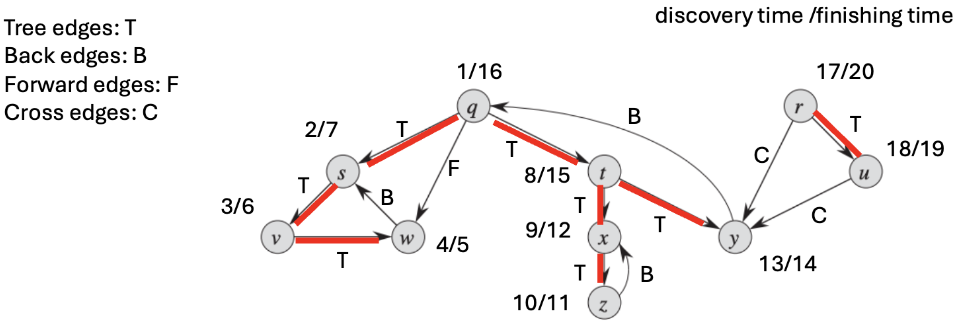
\includegraphics[width=\linewidth]{dfs.png}
    \begin{equation*}
        \left(q\left[s\{v(ww)v\}s\right][t\{x(zz)x\}yyt]q\right)(r[uu]r)
    \end{equation*}
    \begin{description}
        \item[Tree Edges] Are edges in depth-first forest \(G_\pi\). Edge \((u, v)\)
            is a tree edge if $v$ was first discovered by exploring edge \((u, v)\)
        \item[Back Edges] Are edges \((u, v)\) connecting a vertex $u$ to an
            ancestor in a depth-first tree. We consider self-loops, which may occur
            in directed graphs, to be back edges.
        \item[Forward Edges] Are nontree edges \((u, v)\) connecting a vertex $u$ to
            a descendant $v$ in a depth-first tree.
        \item[Cross Edges] Are all other edges. They can go between vertices in the
            same depth-first tree, as long as one vertex is not an ancestor of the
            other, or they can go between verticies in different depth-first trees.
    \end{description}

    \subsection*{Graphs}
    \subsubsection*{Handshaking Lemma}
    \begin{equation*}
        \sum_{v \in V} \text{deg}(v) = 2|E|
    \end{equation*}

    \subsection*{BFS vs DFS}
    \begin{itemize}
        \item DFS is usually for finding relationship among vertices.
        \item BFS Is usually for finding shortest path from a given source.
    \end{itemize}

    % \newpage
    % \pagebreak
    \subsection*{Djikstra}
    Execute Djikstra's algorithm on the graph below starting at A. If there are
    ties, the vertex with the lowest letter comes first.
    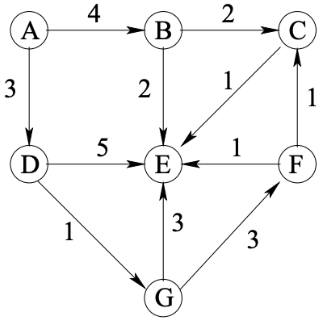
\includegraphics[width=0.5\columnwidth]{djikstra.png}
    \begin{tabular}{ccccccc}
        A: 0          & D: 3          & B: 4          & G: 4          & C: 6 &
        E: 6          & F: 7                                                   \\
        B: \(\infty\) & B: 4          & G: 4          & C: 6          & E: 6 &
        F: 7                                                                   \\
        C: \(\infty\) & C: \(\infty\) & E: 8          & E:6           & F: 7
        \\
        D: \(\infty\) & E: \(\infty\) & C: \(\infty\) & F: \(\infty\)
        \\
        E: \(\infty\) & F: \(\infty\) & F: \(\infty\)
        \\
        F: \(\infty\) & G: \(\infty\)
        \\
        G: \(\infty\)
    \end{tabular}
    \columnbreak
    \subsection*{Floyd-Warshall}
    Execute the Floyd-Warshall algorithm on the graph below, provide the \(D^k\)
    and \(P\) matrixes on each step.
    \begin{center}
        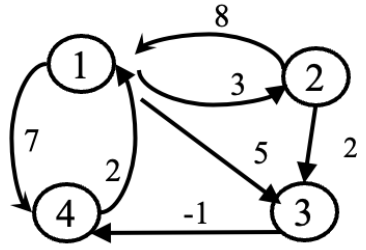
\includegraphics[width=0.75\columnwidth]{floyd.png}
    \end{center}
    \begin{align*}
        D^0 & = \begin{array}{c|cccc}
                      & 1      & 2      & 3      & 4      \\
                    \hline
                    1 & 0      & 3      & 5      & 7      \\
                    2 & 8      & 0      & 2      & \infty \\
                    3 & \infty & \infty & 0      & -1     \\
                    4 & 2      & \infty & \infty & 0
                \end{array}
            & P = \begin{array}{c|cccc}
                        & 1 & 2 & 3 & 4 \\
                      \hline
                      1 & 0 & 0 & 0 & 0 \\
                      2 & 0 & 0 & 0 & 0 \\
                      3 & 0 & 0 & 0 & 0 \\
                      4 & 0 & 0 & 0 & 0
                  \end{array}                \\
        D^1 & = \begin{array}{c|cccc}
                      & 1      & 2      & 3 & 4  \\
                    \hline
                    1 & 0      & 3      & 5 & 7  \\
                    2 & 8      & 0      & 2 & 15 \\
                    3 & \infty & \infty & 0 & -1 \\
                    4 & 2      & 5      & 7 & 0
                \end{array}
            & P = \begin{array}{c|cccc}
                        & 1 & 2 & 3 & 4 \\
                      \hline
                      1 & 0 & 0 & 0 & 0 \\
                      2 & 0 & 0 & 0 & 1 \\
                      3 & 0 & 0 & 0 & 0 \\
                      4 & 0 & 1 & 1 & 0
                  \end{array}                \\
        D^2 & = \begin{array}{c|cccc}
                      & 1      & 2      & 3 & 4  \\
                    \hline
                    1 & 0      & 3      & 5 & 7  \\
                    2 & 8      & 0      & 2 & 15 \\
                    3 & \infty & \infty & 0 & -1 \\
                    4 & 2      & 5      & 7 & 0
                \end{array}
            & P = \begin{array}{c|cccc}
                        & 1 & 2 & 3 & 4 \\
                      \hline
                      1 & 0 & 0 & 0 & 0 \\
                      2 & 0 & 0 & 0 & 1 \\
                      3 & 0 & 0 & 0 & 0 \\
                      4 & 0 & 1 & 1 & 0
                  \end{array}                \\
        D^3 & = \begin{array}{c|cccc}
                      & 1      & 2      & 3 & 4  \\
                    \hline
                    1 & 0      & 3      & 5 & 4  \\
                    2 & 8      & 0      & 2 & 1  \\
                    3 & \infty & \infty & 0 & -1 \\
                    4 & 2      & 5      & 7 & 0
                \end{array}
            & P = \begin{array}{c|cccc}
                        & 1 & 2 & 3 & 4 \\
                      \hline
                      1 & 0 & 0 & 0 & 3 \\
                      2 & 0 & 0 & 0 & 3 \\
                      3 & 0 & 0 & 0 & 0 \\
                      4 & 0 & 1 & 1 & 0
                  \end{array}                \\
        D^4 & = \begin{array}{c|cccc}
                      & 1 & 2 & 3 & 4  \\
                    \hline
                    1 & 0 & 3 & 5 & 4  \\
                    2 & 3 & 0 & 2 & 1  \\
                    3 & 1 & 4 & 0 & -1 \\
                    4 & 2 & 5 & 7 & 0
                \end{array}
            & P = \begin{array}{c|cccc}
                        & 1 & 2 & 3 & 4 \\
                      \hline
                      1 & 0 & 0 & 0 & 3 \\
                      2 & 4 & 0 & 0 & 3 \\
                      3 & 4 & 4 & 0 & 0 \\
                      4 & 0 & 1 & 1 & 0
                  \end{array}                \\
    \end{align*}

    \subsection*{Knapsack}
    \begin{equation*}
        c[i, w] = \begin{cases}
            0                                    & \text{if } i = 0 \text{ or } w = 0 \\
            c[i-1, w]                            & \text{if } w_i > w                 \\
            \max(c[i-1, w], c[i-1, w-w_i] + v_i) & \text{otherwise}
        \end{cases}
    \end{equation*}
\end{multicols*}
\end{document}